\documentclass{beamer}
\usepackage[utf8]{inputenc}
\usetheme[background=dark,titleformat = smallcaps , block = fill,numbering = fraction, progressbar = frametitle , titleformat title= smallcaps]{metropolis}           % Use metropolis theme


\definecolor{orangeBar}{HTML}{FF3600}
\setbeamercolor{progress bar}{fg=orangeBar}

\usepackage {extarrows}
\usepackage {tikz}
\usepackage[spanish]{babel}
\usepackage{graphicx}
\usepackage{amssymb}
%\usepackage{amsfonts}

\usepackage{enumerate}
\usepackage{amsmath}
\usepackage{amsthm}
\usepackage{xcolor}
%\usepackage{amsfonts,amssymb,amsthm}

\usepackage{url}
\usepackage{enumerate}
\usepackage{commath}
\usepackage{multicol}
\usepackage{mathtools}
\usepackage{scrextend}
\usepackage{hyperref}
\usepackage{cleveref}
\usepackage{longtable}
\usepackage{bbm}
\usepackage{siunitx}
\usepackage{listings}
\usepackage{xcolor}
\usepackage{subcaption}
\usepackage{epigraph}


\definecolor{codegreen}{rgb}{0,0.6,0}
\definecolor{codegray}{rgb}{0.5,0.5,0.5}
\definecolor{codepurple}{rgb}{0.58,0,0.82}
\definecolor{backcolour}{rgb}{0.95,0.95,0.92}

\lstdefinestyle{mystyle}{
	backgroundcolor=\color{backcolour},   
	commentstyle=\color{codegreen},
	keywordstyle=\color{blue},
	numberstyle=\tiny\color{codegray},
	stringstyle=\color{red},
	basicstyle=\ttfamily\footnotesize,
	breakatwhitespace=false,         
	breaklines=true,                 
	captionpos=b,                    
	keepspaces=true,                 
	numbers=left,                    
	numbersep=5pt,                  
	showspaces=false,                
	showstringspaces=false,
	showtabs=false,                  
	tabsize=2
}

\lstset{style=mystyle}
\lstset{language=Python}
\lstset{frame=lines}
\lstset{caption={Insert code directly in your document}}
\lstset{label={lst:code_direct}}
\lstset{basicstyle=\footnotesize}


\newcommand{\bb}[1]{\mathbb{#1}}

%\newtheorem{theorem}{Teorema}[section]
%\theoremstyle{plain}
\newtheorem{acknowledgement}[theorem]{Acknowledgement}
\newtheorem{algorithm}[theorem]{Algorithm}
\newtheorem{axiom}[theorem]{Axiom}
\newtheorem{case}[theorem]{Case}
\newtheorem{claim}{Claim}
\newtheorem{conclution}[theorem]{Conclusión}
\newtheorem{condition}[theorem]{Condition}
\newtheorem{conjecture}[theorem]{Conjecture}
%\newtheorem{corollary}[theorem]{Corolario}
\newtheorem{criterion}[theorem]{Criterion}
\theoremstyle{definition}
%\newtheorem*{df}{Definición}
%\newtheorem{definition}[theorem]{Definición}
%\newtheorem{example}[theorem]{Ejemplo}
\newtheorem{exercise}[theorem]{Exercise}
%\newtheorem{lemma}[theorem]{Lema}
\newtheorem{notation}[theorem]{Notation}
%\newtheorem{problem}[theorem]{Problem}
\newtheorem{proposition}[theorem]{Proposición}
\newtheorem{remark}[theorem]{Nota}
%\newtheorem{solution}[theorem]{Solución}
\newtheorem{summary}[theorem]{Summary}
\numberwithin{equation}{section}

\definecolor{defColor}{HTML}{3ED597}
\newcommand{\marine}[1]{\textcolor{defColor}{#1}}


\definecolor{thColor}{HTML}{FA7E0A}
\newcommand{\orangee}[1]{\textcolor{thColor}{#1}}

\definecolor{rkColor}{HTML}{F72121}
\newcommand{\redd}[1]{\textcolor{rkColor}{#1}}




\newtheorem{df}{\marine{Definición}}
\newtheorem{thh}{\orangee{Teorema}}
\newtheorem{pr}{\orangee{Proposición}}
\newtheorem{lm}{\orangee{Lema}}
\newtheorem{crr}{\orangee{Corolario}}
\newtheorem{rr}{\redd{Observación}}


%\newtheorem{defn}[]{Definición}
%\newenvironment{definition}{\begin{defn}}{\end{defn}}
%\newtheorem{definition}{Definition}[section]
%\newtheorem*{remark}{Remark}
%%%%%%%%
\newcommand{\tit}[1]{\textit{#1}}
\newcommand{\bsym}{\mathbf}
\newcommand{\Mod}[1]{\ (\mathrm{mod}\ #1)}
%\newcommand{\blue}[1]{\textcolor{blue}{#1}}
\newcommand{\red}[1]{\textcolor{red}{#1}}
\renewcommand{\geq}{\geqslant}
\renewcommand{\leq}{\leqslant}
\newcommand{\Rplus}{\mathds{R}_{^{+}}}
\newcommand{\N}{\mathbb{N}}
\newcommand{\Z}{\mathbb{Z}}
\newcommand{\R}{\mathbb{R}}
\newcommand{\C}{\mathbb{C}}
\newcommand{\Q}{\mathbb{Q}}
\newcommand{\ssi}{\longleftrightarrow}
\newcommand{\ent}{\longrightarrow}
\newcommand{\Qp}{\mathbb{Q}_p}  
\newcommand{\Qpn}{\mathbb{Q}_p^n}
\newcommand{\Zpn}{\mathbb{Z}_p^n}
\newcommand{\Zp}{\mathbb{Z}_p}
\newcommand{\Zd}{\mathbb{Z}_2}
%\newcommand{\abs}[1]{\left\vert #1 \right\vert}
%\newcommand{\norm}[1]{\|#1\|}
\newcommand{\pnorm}[1]{\|#1\|_p}
\newcommand{\maxx}[1]{\text{m\'ax} #1}
\newcommand{\xbar}[1]{\hskip 1.4pt\overline{\hskip-1.2pt #1\hskip -.6pt}\hskip 1.2pt}
\newcommand{\rb}{\raisebox{-.35ex}}

\DeclareMathOperator{\s}{\mathbf{S}}
\DeclareMathOperator{\f}{\mathcal{F}}
\DeclareMathOperator{\A}{\mathbb{A}}
\DeclareMathOperator{\dist}{dist} % The distance.
\DeclareMathOperator{\d^n}{\dif^{\,n}}
%\DeclareMathOperator{\d}{\dif}
\DeclareMathOperator{\Real}{Re}
\DeclareMathOperator{\ord}{Ord}
\DeclareMathOperator{\Dom}{Dom}
\DeclareMathOperator{\vol}{vol}
\DeclareMathOperator{\gpn}{\mathit{{GpnN}}}
%%%%%%%%%
%%%%%%%%%%%%%%%%% dashed integrals %%%%%%%%%%%%%%%%%%%%%
\DeclareSymbolFont{eulargesymbols}{U}{zeuex}{m}{n}
\DeclareMathSymbol{\intop}{\mathop}{eulargesymbols}{"52}
\usepackage[toc,page]{appendix}
\renewcommand{\labelitemi}{$\circ$}


\title{Una introducción a los números $p$-ádicos, su aritmética y algunas simulaciones en \textit{Python}}
\subtitle{Trabajo de grado presentado para optar por el título de
Matemático}
\date{\today}


\author{\bf{Autor: }Edgar Baquero 
	\\ \bf{Supervisor: }Leonardo Chacón. PhD.}

\institute{Pontificia Universidad Javeriana,
Facultad de Ciencias\\
Departamento de Matemáticas}
\begin{document}
  \maketitle
  \section{Notación}
  \begin{frame}{Unidades, decenas y centenas...}
    En la escuela nos enseñaron a separar los números por unidades, decenas y centenas. Por ejemplo el número $437$ tiene $7$ unidades, $3$ decenas y $4$ centenas. Es decir que podemos representar $437$ como:
    $$437 = 7\cdot10^0+ 3\cdot 10^1 + 4\cdot 10^2,$$
    El número $543.89$ como:
    $$543.89 = 9\cdot10^{-2}+8\cdot10^{-1}+3\cdot10^0+4\cdot10^1+5\cdot10^2.$$
    Que también se puede denotar como $543.89_{10}$.
  \end{frame}

  \begin{frame}{Sistemas numéricos}
  	Así:
  	\begin{itemize}
  		\item Se puede expandir un número por cualquier base $q$.
 		\item Ejemplos conocidos de sistemas de numeración son el \tit{octal, hexadecimal y binario}, entre otros.
  	\end{itemize}
  \begin{exampleblock}{Ejemplo}
	Podemos representar el siguiente número:
	$$2\cdot8^{-2}+2\cdot8^{-1}+3\cdot8^0+4\cdot8^1+7\cdot8^2,$$
	por $743.22$ ($q=8$), o también $743.22_8$.
  \end{exampleblock}
	 
  \end{frame}

%3------------------
\begin{frame}{Representación que usamos}
	\begin{itemize}[<+- | alert@+>]
		\item Particularmente, estamos interesados en expansiones sobre bases primas.
		\item Por ejemplo con $p=2$, el ¡Sistema binario!
		\item En general, una expansión de la forma.	$$x=\sum_{k=-\gamma}^{l}a_kp^k,\text{ con $\gamma\in\Z$, $a_k\in \{0,\dots,p-1\}$ },$$
		será
		\begin{equation}\label{notacion}
		{a_{l} \ldots a_{2} a_{1} a_{0},a_{-1}a_{-2}\cdots a_{-\gamma}}_p.
		\end{equation}
		\item ¿Deberíamos llamar a las expansiones, expansiones pesimales?
		\item Ni idea. Usaremos los términos: expansión (representación) $p$-ádica ó \tit{Código de Hensel}.
		\item Siendo así, ahora sí empecemos.
	\end{itemize}

\end{frame}
%4-------------------
\section{El campo de los números $p$-ádicos}
\begin{frame}{Norma}
\begin{df}\label{pnorm}
	Sea $K$ un cuerpo. Una \textit{norma} en $K$ es una función
	$\abs{\cdot}\colon K \to \R_{\geq 0}$ tal que para todo $x,y\in$ $K$
	satisface las siguientes propiedades:
	
	\begin{itemize}[<+- | alert@+>]
		\item[$\diamond$] $\abs{x} \geq0$, $\abs{x}
		=0\Longleftrightarrow x=0,$
		
		\item[$\diamond$] $\abs{xy}  =\abs{x} \left\vert 
		y\right\vert ,$
		
		\item[$\diamond$] $\left\vert x+y\right\vert \leq\abs{x} +\left\vert y\right\vert$.
	\end{itemize}
\end{df}
	Además, una norma $\abs{\cdot}$ en $K$ define una métrica natural dada por\linebreak ${d (x,y)=\abs{x-y}}$.
\end{frame}
%5-----------------------------------------
\begin{frame}{Equivalencia entre normas}
\begin{df}
	Dos normas $\abs{\cdot}_1$, $\abs{\cdot}_2$ sobre un cuerpo $K$ se dicen \tit{equivalentes }si inducen la misma topología sobre $K$, i.e., todo abierto con respecto a una  topología también  lo es con respecto a la otra. Por notación decimos que $\abs{\cdot}_1\sim\abs{\cdot}_2$.
\end{df}

\begin{pr}\label{quiv_power}
	Sea $K$ un cuerpo con dos normas $\abs{\cdot}_1$, $\abs{\cdot}_2$. Entonces \linebreak$\abs{\cdot}_1\sim\abs{\cdot}_2$ si, y sólo si, existe $c\in\bb{R}_{>0}$ tal que $\abs{\cdot}_1=\abs{\cdot}_2^c$.
\end{pr}
\end{frame}
%6----------------------
\begin{frame}{Equivalencia entre normas}
\begin{pr}
	[Equivalencia Lipschitz ]\label{lipeq}
	Sea $K$ un cuerpo con dos normas $\abs{\cdot}_1$, $\abs{\cdot}_2$. Entonces $\abs{\cdot}_1\sim\abs{\cdot}_2$ si, y sólo si existen constantes $k_1,k_2$ positivas tales que:
	$$k_1\abs{x}_1<\abs{x}_2< k_2\abs{x}_1,$$
	para todo $x\in K$.
\end{pr}
\begin{pr}
	\label{equiv_cauchy}
	Sea $K$ un cuerpo con dos normas $\abs{\cdot}_1$, $\abs{\cdot}_2$ tales que ${\abs{\cdot}_1\sim\abs{\cdot}_2}$, entonces una sucesión $ (x_n)$ es de Cauchy respecto a $\abs{\cdot}_1$ si, y sólo si es de Cauchy respecto a $\abs{\cdot}_2$.
\end{pr}
\end{frame}

%7----------------------
\begin{frame}{Norma no-arquimediana}
\begin{df}
	Una norma $\norm{\cdot}$ sobre un cuerpo $K$ se dice \textit{no-arquimediana o ultramétrica}, si la condición $ (3)$  (en la definición \ref{pnorm})  es reemplazada por
	\begin{equation}\label{condiultra}
	\|x+y\| \le \maxx\{\|x\|, \|y\|\}, \forall x,y\in K.
	\end{equation} 
\end{df}
\begin{rr}
	Dado que
	$$\|x+y\| \le \maxx\{\|x\|, \|y\|\} \leq \|x\| + \|y\|, \forall x,y\in \mathbb{Q},$$ 
	la condición \ref{condiultra} es también llamada \tit{desigualdad triangular  fuerte}.
\end{rr}
\end{frame}

%8----------------------
\begin{frame}{Orden y Norma en $\Q$}
\begin{df} \label{ord_def_1}
	Fijemos un primo $p$, sea $x\in\mathbb{Q\smallsetminus}\left\{  0\right\}  $ expresado de forma única como $x=p^{v}\frac{a}{b}$, donde $v$ es un entero y
	$a$, $b$ son  primos relativos con $p$.
	Definimos la función $\pnorm{\cdot}$ de la siguiente manera:
	\[
	\| x\| _{p}=p^{-v},
	\]
	donde el entero $v=v\left (  x\right)  $ se denomina el orden $p$\textit{-ádico de} $x$ y
	será denotado por $\ord\left (  x\right)  $. Por definición $\|0\|_p=0$, y  $\ord (0)=+\infty $.
\end{df}
\end{frame}
%9----------------------
\begin{frame}{Orden y Norma en $\Q$}
	\begin{exampleblock}{Ejemplo}
		Cálculo de la función $\pnorm{\cdot}$ para distintos $p$'s.
		\[
		\left| -\frac{66}{500}\right| _{p}=\left| -\frac{33}{250}\right| _{p}=\left| -\frac{3\cdot11}{2\cdot5^3}\right| _{p}=\begin{cases}
		\frac{33}{250}       &\,\,\, \text{ si } \,\,\,p=\infty;\\ 
		2                    &\,\,\, \text{ si }\,\,\, p=2;\\
		\frac{1}{3}          &\,\,\, \text{ si } \,\,\,p=3;\\  
		5^3                  &\,\,\, \text{ si }\,\,\, p=5;\\   
		1                    &\,\,\, \text{ si }\,\,\, p=7;\\    
		\frac{1}{11}         & \,\,\,\text{ si }\,\,\, p=11;\\     
		& \vdots\\
		1                   &\,\,\,\text{ otro caso}.
		\end{cases}
		\]
	\end{exampleblock}
\end{frame}
%10-----------------------------------------------
\begin{frame}{Los 3 mosqueteros}
	
	\begin{thh}
		[\tit{Fórmula Adélica del producto}]
		Sea $x\in \bb{Q}$ tal que $x\neq0$, entonces:
		$$\displaystyle\prod_{p}^\infty \norm{x}_p=1, \text{ con } \norm{x}_\infty=\abs{x} \text{ y $p$ primo}.$$
	\end{thh}
\begin{thh}
		$\| \cdot \|_p$ es una norma no arquimediana.	
\end{thh}
\begin{thh}
	[Ostrowski]	\label{ostrowsky} Cualquier norma no trivial sobre $\mathbb{Q}$ es equivalente al
	valor absoluto usual, o a una norma p-ádica $\| \cdot\| _{p}%
	$, para algún primo $p$.
\end{thh}
\end{frame}
%11-----------------------------------------------
\begin{frame}{No equivalencia de normas en $\Q$}
	\begin{rr}
			Las normas $\norm{\cdot}_p$ y $\norm{\cdot}_q$ no son quivalentes si $p$ y $q$ son primos distintos. Por ejemplo, sea $p=5$ y $q=7$, la sucesión 
		$x_n=\big (\frac{5}{7}\big)^n$ se tiene que 
		$$\norm{x_n}_5=5^{-n}\rightarrow 0 \text{ y } \norm{x_n}_7=7^{n}\rightarrow \infty ,$$
		cuando $n \rightarrow \infty$.
		
		El valor absoluto usual sobre $\Q$ tampoco es equivalente a una norma $p$-ádica. Por ejemplo, considérese la sucesión $x_n= (\frac{1}{p})^n$, entonces
		$$\abs{x_n}=p^{-n}\to 0 \text{ y } \norm{x_n}_p = p^n \to \infty,$$
		cuando $n\to\infty$. Lo cual contradice la proposición \ref{equiv_cauchy}.
	\end{rr}
\end{frame}
%12-----------------------------------------------
\begin{frame}{Sucesiones de Cauchy}
\begin{thh}
	[Caracterización de sucesiones de Cauchy]\label{car}
	Una sucesión $ (x_n)_{n\in\N}$ en $\Q$ es de Cauchy, si, y sólo si:
	\begin{equation}\label{car_cau}
	\lim_{n\to\infty}\pnorm{x_{n+1}-x_n}=0.
	\end{equation}
\end{thh}
\begin{df}
	Sea $ (\bb{K}, \norm{\cdot})$ un cuerpo métrico. Sea ${\bb{K}^\N}$ el anillo de todas las sucesiones en $\bb{K}$. Definimos $\mathcal C,\mathcal N $ como el subanillo de todas las sucesiones de Cauchy y el subanillo de todas las sucesiones finalmente nulas, respectivamente.
\end{df}
\end{frame}
%14-----------------------------------------------
\begin{frame}{Completación de un cuerpo métrico}
\begin{df}
	[Completación de un cuerpo métrico]Sea $ (\bb{K}, \norm{\cdot})$ un cuerpo métrico. Sean $\mathcal C,\mathcal N $ los subanillos de todas las sucesiones de Cauchy y de todas las sucesiones finalmente nulas, respectivamente.  Definimos el cociente de anillos $\hat{\bb{K}}\coloneqq \mathcal C/\mathcal N  $ como la completación de $\bb{K}$.
\end{df}
\begin{rr}
	La norma $\norm{\cdot}\colon{\hat{\bb{K}}}\to\R_+,$ sobre la completación de $\bb{K}$ está definida tal que para todo $ (x_n)+\mathcal{N} \in \hat{\bb{K}}$:
	$$\norm{ (x_n)+\mathcal{N}}=\lim_{n\to\infty}\norm{x_n}.$$
\end{rr}
\end{frame}

\begin{frame}{Completaciones de $\Qp$}
	\begin{figure}
		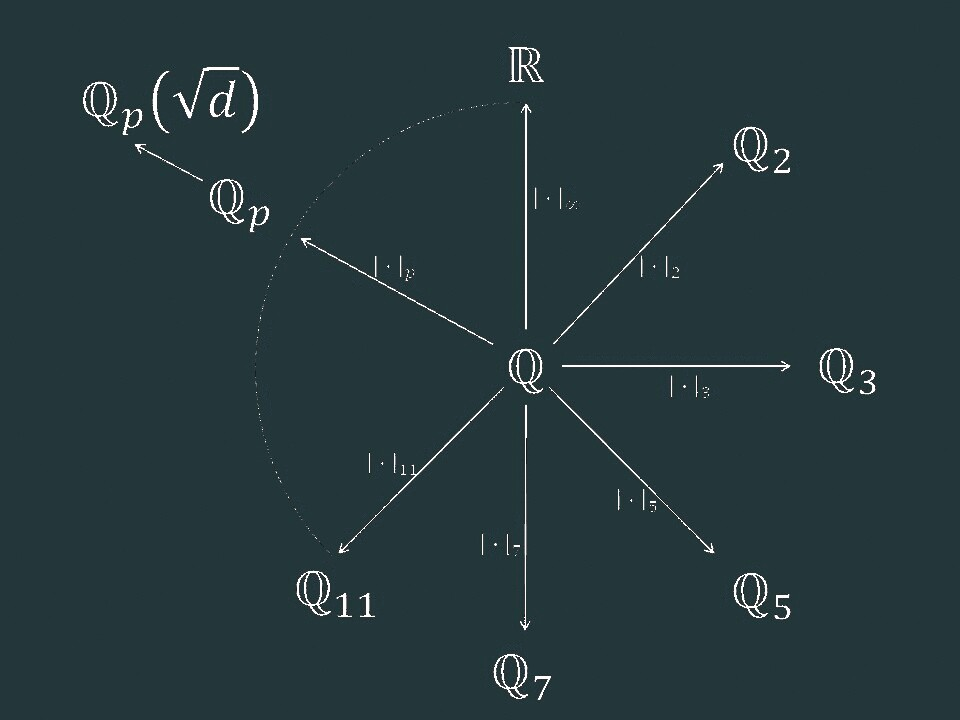
\includegraphics[scale=0.35]{img/relojBeamer.jpg}\caption{Completaciones respecto a las distintas normas en $\Q$}
	\end{figure}
\end{frame}
%15-----------------------------------------------
\begin{frame}{$\Q$ no es completo :c}
	El siguiente teorema es importante, pues caracteriza a $\Q$ como un cuerpo no completo.
	\begin{thh}
		$ (\Q, d (x,y)=\pnorm{x-y})$ y $ (\Q, d (x,y)=|x-y|)$ no son espacios completos.
	\end{thh}
\begin{exampleblock}{Ejemplo}
	Un procedimiento para construir una sucesión de Cauchy en $ (\Q, d (x,y)=\pnorm{x-y})$ podría hacerse, tomando $a\in\Q$ tal que:
	\begin{itemize}[<+- | alert@+>]
		\item[$\diamond$] $a$ no es cuadrado en $\Q$
		\item[$\diamond$] $p \nmid a$
		\item[$\diamond$] $a$ es residuo cuadrático módulo $p$. i.e., $x^2 \equiv a \Mod{p^n}$ tiene solución.
	\end{itemize}
\end{exampleblock}
\end{frame}


%16-----------------------------------------------
\begin{frame}{$\Q$ no es completo :c}
	\begin{exampleblock}{Continuación$\dots$}
		Podemos hallar $a$ tal que sea cuadrado en $\Z$ y sumarle un múltplo de $p$; para así construir la sucesión como sigue:
		\begin{itemize}[<+- | alert@+>]
			\item[$\diamond$] Tomamos $x_0$ solución de $x^2\equiv a \Mod{p}$
			\item[$\diamond$] Construimos a $x_1$ tal que $x_1 \equiv x_0 \Mod{p}$ y además ${x_1^2\equiv a \Mod{p^2}}$ 
			\item[$\diamond$] Recursivamente, construimos $x_n$ tal que:
			$$x_n \equiv x_{n-1} \Mod{p^n} \text{ y } {x_n^2\equiv a \Mod{p^{n+1}}}$$
		\end{itemize}
	Es de cauchy: $  \pnorm{x_{n+1}-x_n} = \pnorm{kp^n} \leq \pnorm{p^n}=p^{-n}\rightarrow0.$\linebreak
	No converge: $\pnorm{x_n^2-a}=\pnorm{sp^{n+1}}\leq \pnorm{p^{n+1}}\leq p^{- (n+1)}\to 0,$
	luego $x_n\to \sqrt{a}\notin\Q$.
	\end{exampleblock}
\end{frame}
%-------------Topology----------------------
\section{Topología en $\Qp$}
%17-----------------------------------------
\begin{frame}{El espacio $\Qpn$}
	Podemos definir en $\Qpn$ una norma como:\[
	\pnorm{x}:=\max_{1\leq i\leq n}\pnorm{x_i},\qquad\text{para }x= (x_{1},\dots,x_{n})\in\Qpn.
	\]
	Así, $(\Qpn, d=\pnorm{x-y})$ es un espacio métrico, donde las distancias están en el conjunto \{$p^\gamma$$\colon$ $\gamma\in\Z$\}$\cup$\{$0$\}. Luego, tiene sentido definir los abiertos básicos por:
	 \[
	 B^n_{\gamma} (a)=\{x\in\Qp:\pnorm{x-a}< p^{\gamma}\},\ \gamma\in \mathbb{Z}.
	 \]
	 \begin{rr}
	 	$B_\gamma^n (a)$ es un grupo aditivo.
	 \end{rr}
\end{frame}
%18-----------------------------------------
\begin{frame}{Algunas propiedades topológicas de $\Qpn$}
	Análogamente pordemos definir la esfera $n$-dimensional con centro en $a$:
	\[
	S^n_{r} (a)=\{x\in\Qpn:\pnorm{x-a}=p^{r}\},\ r\in \mathbb{Z}.
	\]
	Además
	\begin{itemize}[<+- | alert@+>]
		\item $S_{\gamma}^n (a)=\left\{x:\pnorm{x-a}=p^{\gamma}\right\}=B_{\gamma}^n (a) \backslash B_{\gamma-1}^n (a).$
		\item${B_{\gamma}^n (a) \subset B_{\gamma^{\prime}}^n (a)}$ siempre que $\gamma<\gamma^{\prime}.$
		\item $B_{\gamma-1}^n (a)=\left\{x:\pnorm{x-a}<p^{\gamma}\right\}.$ 
		\item $B_{\gamma}^n (a)=\bigcup_{\gamma^{\prime} \leq \gamma} S_{\gamma^{\prime}}^n (a).$
		\item $\bigcup_{\gamma} B_{\gamma}^n (a)=\bigcup_{\gamma} S_{\gamma}^n (a)=\mathbb{Q}_{p}^n-\{0\}.$
		\item $\bigcap_{\gamma} B_{\gamma}^n (a)=\{a\}.$
	\end{itemize}
\end{frame}
%18-----------------------------------------
\begin{frame}{Propiedades bonitas de $\Qp$ :o}
	\begin{thh}
	\begin{itemize}[<+- | alert@+>]
		\item \label{clopen1} Si $b\in B_{r} (a)$, entonces $B_{r} (a)=B_{r} (b)$. En otras palabras: ¡Todo  punto de una bola abierta es centro de la misma!
		\item Toda bola es a su vez, un conjunto cerrado y abierto.
		\item Dos bolas en $\Qp$ son disyuntas o una contiene a la otra; es decir, si $a,b \in \bb{Q}_p$, y $r,s\in \Z$, se tiene que $B_{r} (a)\cap B_{s} (b)\neq\emptyset$ si, y sólo si, $B_{r} (a)\subseteq B_{s} (b)$ o $B_{s} (b)\subseteq B_{r} (a)$.
	\end{itemize}	
	\end{thh}
	
	
\end{frame}

%19-----------------------------------------
\begin{frame}{Más propiedades de $\Qp$ }
\begin{thh}
	$\Qp$ es un espacio de \tit{Hausdorff}
\end{thh}
\begin{thh}
	$\{B_\gamma (a)\colon r\in\Z, a\in\Qp\}$ es contable.
\end{thh}
\begin{thh}
	$\Qp$ es un espacio localmente compacto.
\end{thh}
	
	
\end{frame}
%20-----------------------------------------
\begin{frame}{Algunas definiciones de Topología}
\begin{df}
		Decimos que un espacio topológico es \tit{conexo} si no puede ser escrito como la unión de dos abiertos disyuntos no vacíos. Por otro lado, decimos que un espacio es \tit{disconexo} si es la unión de dos abiertos disyuntos no vacíos.
\end{df}

\begin{df}
Los subconjuntos conexos maximales de un espacio topológico son llamados \tit{componentes conexos}.
\end{df}

\begin{df}
	Decimos que un espacio topológico es \tit{totalmente disconexo} si todas sus componentes conexos son singletons.
\end{df}
	
\end{frame}

%21-----------------------------------------
\begin{frame}{Un corolario simple y bonito}
	\begin{thh}
		$\Qp$ es totalmente disconexo.
	\end{thh}
	\begin{thh}
		$\N$ es denso en $\Zp$.
	\end{thh}
	\begin{lm}
		Sean $x, y \in \bb{Q}_p$ tales que $\norm{x}_p \neq \norm{y}_p.$ Entonces:
		$$\norm{x+y}_p=\maxx\{\norm{x}_p,\norm{y}_p\}$$
	\end{lm}
	\begin{crr}
		Todos los triángulos en $\Qp$ son isósceles.  
	\end{crr}
\end{frame}
%22-----------------------------------------
\begin{frame}{Un corolario simple y bonito}

\begin{figure}
	\centering
	\begin{tikzpicture}
	
	%   \draw [black!20]  (0,0) grid  (3,4);
	\draw[black]  (0,0)-- (3,0)--  (1.5,4)--cycle;
	
	
	\draw  (0,0) circle  (0pt) node[anchor=north] {$y$};
	\draw  (3,0) circle  (0pt) node[anchor=north] {$z$};
	\draw  (1.5,4.5) circle  (0pt) node[anchor=north] {$x$};
	\draw  (3.5,2) circle  (0pt) node[anchor=north] {$\pnorm{x-z}$};
	\draw  (-0.5,2) circle  (0pt) node[anchor=north] {$\pnorm{x-y}$};
	\draw  (1.5,-0.2) circle  (0pt) node[anchor=north] {$\pnorm{z-y}$};  
	\end{tikzpicture}
	\caption{Todos los triángulos en $\bb{Q}_p$ son isósceles}
	\label{fig:1}
\end{figure}
\end{frame}
%24-----------------------------------------
\begin{frame}{Relación de $\Qp$ con $\R$}
\begin{itemize}
	\item Existe una correspondencia con los \textit{Conjuntos de Cantor}.
	\item También podemos relacionarlos mediante una función $\rho\colon\Qp\to\R_{+}$ conocida como \textit{Monna map}, definida por
	\begin{equation}\label{Monna}
	\rho: \sum_{j=\gamma}^{\infty} x_{j} p^{j} \mapsto \sum_{j=\gamma}^{\infty} x_{j} p^{-j-1}, \quad x_{j}=0,1, \ldots, p-1, \quad \gamma \in \mathbb{Z},
	\end{equation}
\end{itemize}
\end{frame}
%25-----------------------------------------
\begin{frame}{Propiedades de $\rho$}
	\begin{itemize}[<+- | alert@+>]
		\item {$\rho$ es una función continua, sobreyectiva, pero no inyectiva.}
		\item $|\rho (x)-\rho (y)| \leq\pnorm{x-y}, \text{ para todo } x, y \in \mathbb{Q}_{p}$.
		Es decir, $\rho$ satisface la desigualdad de Hölder,
		\item $\rho\left (p^{\gamma} x\right)=p^{-\gamma} \rho (x), \text{ para todo }x \in \mathbb{Q}_{p}.$
	\end{itemize}
\end{frame}
%------------------------Arithmetic------------------------
\section{Aritmética $p$-ádica}

\begin{frame}{Expansiones $p$-ádicas de enteros}
	\begin{itemize}[<+- | alert@+>]
		\item Podemos expandir por cualquier base $p$ un número $n\in\Z$
		\item El procedimiento es algorítmico:
		$$a_0 =n\bmod p\hspace{5mm} \Longrightarrow \hspace{5mm} n_1 = \frac{n-a_0}{p},$$ $$a_1 =n_1\bmod p \hspace{5mm} \Longrightarrow \hspace{5mm} n_2 = \frac{n_1-a_1}{p},$$ $$a_2 =n_2\bmod p \hspace{5mm} \Longrightarrow \hspace{5mm} n_3 = \frac{n_2-a_2}{p},$$
		$$\vdots$$
		\item Así, la representación de un entero $p$-ádico por dígitos está dada por \ref{notacion}
		$$n={ a_{l} \ldots a_{3} a_{2} a_{1} a_{0}}_p,$$
		\item La representación es conocida como el \textit{Código de Hensel} de $n$.
	\end{itemize}
\end{frame}

\begin{frame}{Expansiones $p$-ádicas de enteros}
\begin{exampleblock}{Ejemplo}
	Sea $n=5353$ y sea $p=5$, entonces la representación $p$-ádica de 5353 en base 5 está dada por:
	\begin{align*}
	%\centering
	a_0 =5353\bmod5 = 3 \hspace{3mm} \Longrightarrow \hspace{3mm} n_1 = \frac{5353-3}{5}=1070,\\
	a_1 =1070\bmod 5=0 \hspace{3mm} \Longrightarrow \hspace{5mm}n_2 = \frac{1070-0}{5}=214,\\
	a_2 =214\bmod 5=4 \hspace{5mm} \Longrightarrow \hspace{9mm}n_3 = \frac{214-4}{5}=42,\\
	a_3 =42 \bmod 5=2 \hspace{7mm} \Longrightarrow \hspace{13mm}n_4 = \frac{42-2}{5}=8,\\
	a_4 =8 \bmod 5=3 \hspace{9mm} \Longrightarrow \hspace{15mm}n_5 = \frac{8-3}{5}=1,\\
	a_5 =1 \bmod 5=1 \hspace{9mm} \Longrightarrow \hspace{15mm}n_6 = \frac{1-1}{5}=0.
	\end{align*}
	En otras palabras, el código de Hensel de $5353$ es $132403_5$.
\end{exampleblock}
\end{frame}

\begin{frame}{Expansiones $p$-ádicas de racionales}
Consideremos $x$ tal que su serie de expansión es
$$
\begin{aligned}
x &=2+3 p+p^{2}+3 p^{3}+p^{4}+3 p^{5}+p^{6}+\cdots \\
&=2+3 p\left (1+p^{2}+p^{4}+\cdots\right)+p^{2}\left (1+p^{2}+p^{4}+\cdots\right) \\
&=2+\left (3 p+p^{2}\right)\left (1+p^{2}+p^{4}+\cdots\right).
\end{aligned}
$$
Como $1+p^{2}+p^{4}+\cdots$ converge a $\left (1-p^{2}\right)^{-1},$ tenemos
$$
x=2+\frac{3 p+p^{2}}{1-p^{2}}.
$$ 
Como caso particular, tomando $p=5$, tenemos que 
$$
x=2+\frac{3\cdot5+5^{2}}{1-5^{2}}=\frac{1}{3},
$$ 
por lo tanto, la expansión $5$-ádica de $\frac{1}{3}$ es $\cdots1313132_5$.
\end{frame}

\begin{frame}{Ejemplos de expansiones $p$-ádicas sobre racionales}
\begin{exampleblock}{Ejemplo}
		\begin{align*}
	&14.31_5=1 \cdot 5^{-2}+3 \cdot 5^{-1}+4 \cdot 5^{0}+1 \cdot 5^{1}=241 / 25 \\
	&1413_5=1 \cdot 5^{0}+3 \cdot 5^{1}+4 \cdot 5^{2}+1 \cdot 5^{3} =241 \\
	&14310_5=0 \cdot 5^{0}+1 \cdot 5^{1}+3 \cdot 5^{2}+4 \cdot 5^{3}+1 \cdot 5^{4}=1205
	\end{align*}
\end{exampleblock}
\end{frame}

\begin{frame}{Suma}
Sean $\alpha= (a_i)$ y $\beta = (b_i)$ dos enteros $p$-ádicos. Definimos la suma como una sucesión $ (c_i)$ de dígitos $p$-ádicos apoyados de una sucesión $ (\epsilon_i)$ en $\{ 0 , 1\}$  (\tit{carries}), tales que:
\begin{itemize}[<+- | alert@+>]
	\item $\epsilon_0=0,$
	\item $c_i=a_i + b_i + \epsilon_i $ ó $c_i=a_i + b_i + \epsilon_i - p$, donde alguno de los dos es un dígito $p$-ádico; es decir, $c_i\in \{0, \dots , p-1\}$. Dado el caso de $c_i$ se tendrá que $\epsilon_{i+1}=0$ o  $\epsilon_{i+1}=1.$
\end{itemize}
\end{frame}

\begin{frame}{Suma}

\begin{exampleblock}{Ejemplo}
	\begin{itemize}
	\item Tomando $p=7$, se tiene: 
	$$
	\vbox{
		\openup2pt
		\def\trule{\noalign{\smallskip\hrule\smallskip}}
		\halign{&\tabskip1em$\mathstrut####$\cr
			& \cdots  & 2 & 5 & 1 & 4 & 1 & 3\cr
			+     & \cdots  & 1 & 2 & 1 & 1 & 0 & 2 \cr
			\trule
			& \cdots  & 4 & 0 & 2 & 5 & 1 & 5 \cr
		}
	}
	%\bye
	$$
	
	\item $0-1$ en los $7$-ádicos: 
	$$
	\vbox{
		\openup2pt
		\def\trule{\noalign{\smallskip\hrule\smallskip}}
		\halign{&\tabskip1em$\mathstrut####$\cr
			& \cdots  & 0 & 0 & 0 & 0 & 0 & 0\cr
			-     & \cdots  & 0 & 0 & 0 & 0 & 0 & 1 \cr
			\trule
			& \cdots  & 6 & 6 & 6 & 6 & 6 & 6 \cr
		}
	}
	%\bye
	$$
	Esto quiere decir que $-1= \cdots 666_7$.
		
	\end{itemize}
	
\end{exampleblock}

\end{frame}

\begin{frame}{Representación de números negativos}
	Si $x=\sum_{i=\gamma}^{\infty}a_ip^i$, entonces $-x=\sum_{i=\gamma}^{\infty}b_ip^i$, donde $b_\gamma = p-a_\gamma$ y\linebreak	 $b_i =  (p-1)-a_i$ con $i>\gamma$.
	
	
	
	\begin{exampleblock}{Ejemplo} Con $p=5$
		\begin{align*}
		&\frac{1}{3}=\cdots1313132_5 \Rightarrow -\frac{1}{3}=\cdots3131313_5,\\
		&\frac{5}{3}=\cdots13131320_5 \Rightarrow -\frac{5}{3}=\cdots31313130_5.
		\end{align*}
	\end{exampleblock}
\end{frame}

\begin{frame}{Numeros unidades}
	\begin{df}
		Un número $p$-ádico es llamado \textit{unidad} si no es múltiplo de una potencia negativa de $p$ y su primer dígito no es $0$.	
	\end{df}
	\begin{exampleblock}{Ejemplo}
		Los números $\cdots314_5$ y $\cdots24_5$ son unidades, mientras que $\cdots310_5$ y $\cdots1321.24_5$ no lo son.	
	\end{exampleblock}
	Así, un número $p$-ádico no-unidad $x=\sum_{j=-N}^{\infty} a_{j} p^{j}$ es un número que puede escribirse de la forma ${x=u\cdot p^{-N}}$ donde $u$ es un número unidad. Por ejemplo
	\begin{align*}
	&\cdots 410_5 = \cdots 41_5\cdot5^1\\
	&\cdots 1321.24_5 = \cdots 132124_5\cdot 5^{-2}.
	\end{align*}
\end{frame}

\begin{frame}{Multiplicación $p$-ádica}
	Sean $x=u\cdot p^{-N_1}$ y $y=v\cdot p^{-N_2}$ con $u,v$ unidades. Definimos la multiplicación $x\cdot y = u\cdot v\cdot p^{- (N_1+N_2)}$
	\begin{exampleblock}{Ejemplo}%\textcolor{red}{corregir este ejemplo, mejor usar la notacion del koblitz y que tengan potencias  negativas}
		\label{mult_ex}
		%Con $p=7$, sea $u = \cdots251413_7$ y $v=\cdots 121102_7$ números unidades. Luego
		$$
		\vbox{
			\openup2pt
			\def\trule{\noalign{\smallskip\hrule\smallskip}}
			\halign{&\tabskip1em$\mathstrut####$\cr
				& \cdots   & 5 & 1 & 4 & 1 & 3\cr
				\times     & \cdots   & 2 & 1 & 1 & 0 & 2\cr
				\trule
				& \cdots   & 3 & 3 & 1 & 2 & 6\cr
				& \cdots   & 0 & 0 & 0 & 0\cr
				& \cdots   & 4 & 1 & 3\cr
				& \cdots   & 1 & 3\cr
				%+ \cdots   & 6\cr
				+          & \cdots  & 6\cr 
				\trule
				& \cdots   & 1 & 0 & 4 & 2 & 6\cr
			}
		}
		%\bye
		$$
		
		Así, con $p=7$, $u\cdot v =\cdots251413_7\times\cdots 123102_7=\cdots 310426_7$.
	\end{exampleblock}
\end{frame}

\begin{frame}{División $p$-ádica}
	Los cálculos de divisiones en los enteros $p$-ádicos no difieren de los métodos tradicionales de división.
	\begin{exampleblock}{Ejemplo}
		%Tomando $p=7$, calculemos $\frac{\cdots421_7}{\cdots153_7}:$
		
		\begin{align*}
		\renewcommand\arraystretch{.75}\renewcommand\arraycolsep{3pt}
		\begin{array}{r@{\hskip\arraycolsep}c@{\hskip\arraycolsep}l*5r} % n=8=3+5
		&&5&1&6\cdots\\
		\cline{2-6} %n=8
		3\hspace{2mm} 5\hspace{2mm} 1&\Big)&1&2&4\cdots \\
		&&1&6&1\cdots \\
		\cline{3-6}\\
		&&&3&2\cdots\\
		&&&3&5\cdots\\
		\cline{4-6}\\
		&&&&4\cdots\\
		&&&&4\cdots\\
		\cline{5-6}\\
		&&&&&\cdots\\
		\end{array}
		\end{align*}
		Así, con $p=7$, $\frac{\cdots421_7}{\cdots153_7}=\cdots 615_7$.
	\end{exampleblock}
\end{frame}

\begin{frame}{División $p$-ádica}
\begin{rr}
	Los anteriores procedimientos de multiplicación y división, hechos sobre $\Zp$ pueden ser extendidos de manera natural a $\Qp$, pues el problema se reduce a operar números unidades.
\end{rr}
\newpage
\begin{exampleblock}{Ejemplo}
	Al momento de multiplicar los números no-unidades, sean 
	\begin{align*}
	&x = \cdots2514.13_7= \cdots251413_7\cdot 7^{-2}=u\cdot 7^{-2},\\
	&y=\cdots 121.102_7=\cdots 121102_7\cdot 7^{-3}=v\cdot 7^{-3},
	\end{align*}
	Luego $$x\cdot y = u\cdot v \cdot 7^{- (2+3)}.$$
	Por el ejemplo \ref{mult_ex}, tenemos que $u\cdot v = \cdots 310426_7$, entonces:
	$$x\cdot y = \cdots 310426_7\cdot 7^{-5}=3.10426_7.$$

	
\end{exampleblock}
\end{frame}
\section{Sucesiones y series de  números $p$-ádicos}

\begin{frame}{Estabilización de sucesiones y series}
\begin{thh}
	Si $$\lim_{n\to\infty}x_n=x, \text{ con } x_n,x\in\Qp\text{ y } \pnorm{x}\neq0 ,$$
	entonces la sucesión $ (\pnorm{x_n})_{n\in\N}$ se estabiliza, es decir, existe $N\in\N$ tal que:
	$$\pnorm{x_n}=\pnorm{x}, \text{ para todo } n\geq N.$$
\end{thh}
\begin{thh}
	Una serie $\sum_{j=1}^\infty x_j, \text{   } x_j\in\Qp$ converge en $\Qp$, si, y sólo si,  $\lim_{n\to\infty}x_n=0$. En tal caso:
	$$\pnorm{\sum_{j=1}^\infty x_j}\leq \maxx_{j}\pnorm{x_j}.$$
\end{thh}
\end{frame}

\begin{frame}{Ejemplos de series}
\begin{exampleblock}{Ejemplo}
	En $\bb{Q}_p$ tenemos que: $$	\sum_{n=1}^{\infty} n^{2}  (n+1) !=2.$$ 
\end{exampleblock}
\begin{block}{Problema abierto}
	Desde el año 1971 se abrió el siguiente problema:
	¿Puede ser $\sum_{n=0}^{\infty}n!$ un número racional para algún primo $p$?
	Por ahora, se sabe que $\sum_{n=0}^{\infty}n!$ converge en cada $\Qp$. Pero nada se sabe de su valor.
\end{block}
\end{frame}

\begin{frame}{Unicidad de la representación}
	\begin{pr}
		Todo número $p$-ádico se puede escribir de manera única como la suma de una serie convergente en  $\Qp$ de la forma:
		\begin{equation}
		\sum_{k=-\infty}^{\infty} a_{k} p^{k}\text{, con $a_k\in\{0,\dots,p-1\}$}	\label{eq:1}
		\end{equation}
		y en donde $a_k=0$, para $k\leq - N$ y $a_{-N}\neq 0$\label{ord_def_2}. A $-N$ se le denomina el \textit{orden} del número.
	\end{pr}
\end{frame}

\begin{frame}{Parte entera y parte fraccionaria}
	\begin{itemize}[<+- | alert@+>]
		
		\item La \textit{\ parte fraccionaria de }$x\in\Qp$, denotada como
		$\left\{  x\right\}  _{p}$, es el siguiente número racional:
		\[
		\left\{  x\right\}  _{p}:=\left\{
		\begin{array}
		[c]{llll}%
		0 & \text{si} & x=0\text{,}  \text{ u}\,  \, \ord (x)\geq0\\
		p^{v}
		{\displaystyle\sum\limits_{j=0}^{\left\vert v\right\vert -1}}
		
		x_{j}p^{j} & \text{si} & \ord (x)<0. &
		\end{array}
		\right.
		\]
		\item Así, para todo $x\in\mathbb{Q}_{p}$ 
		\begin{align*}
		x & =\sum_{i=v}^{-1}a_{i}p^{i}+\sum_{i=0}^{\infty}a_{i}p^{i}\\
		& =:\left\{ x\right\} _{p}+[x]_{p}.
		\end{align*}
	\end{itemize}

\end{frame}

\section{Una mirada algebraica de los números $p$-ádicos}

\begin{frame}{Los enteros $p$-ádicos}
	\begin{df}
		El conjunto
		\[
		\mathbb{Z}_{p} =\{x\in\Qp:|x|_{p}\leq1\}=\{x\in\Qp:x=\sum_{i=i_{0}}^{\infty} a_{i}p^{i},i_{0}\geq0\},
		\]
		es llamado el conjunto de los \textit{enteros $p$-ádicos}.
	\end{df}
\begin{thh}
	$\Zp$ es un subanillo de $\Qp$.
\end{thh}
\end{frame}

\begin{frame}{Números invertibles}
\begin{pr}
	Un entero $p$-ádico $x=\sum_{i=i_{0}}^{\infty}a_{i}p^{i},i_{0}\geq0$ es invertible en $\Zp$ si, y sólo si, $a_0\neq 0$.
\end{pr}
\begin{itemize}
	\item Así, el grupo de los números invertibles en $\Zp$ está dado por:
	$$
	\mathbb{Z}_{p}^{\times}=\left\{x \in \mathbb{Z}_{p}:\pnorm{x}=1\right\}=\Big\{x \in \mathbb{Z}_{p}: x=\sum_{k=0}^{\infty} x_{k} p^{k}, \quad x_{0} \neq 0\Big\},$$
	que es un grupo multiplicativo del anillo $\Zp$.
	\item Estos elementos son llamados \tit{unidades} de $\Qp$ ¡Tal como lo vimos en la sección de aritmética!
\end{itemize}
\begin{exampleblock}{Ejemplo}
	$1-p$ es invertible en $\Zp$, pues su inverso es $\sum_{k=0}^{\infty}p^k=\frac{1}{1-p}.$
\end{exampleblock}
\end{frame}

\begin{frame}{Ideales en $\Zp$}
	\begin{itemize}[<+- | alert@+>]
		\item El anillo $\Zp$ es un \textit{dominio de ideales principales}.
		\item Más exactamente, cualquier ideal de $\mathbb{Z}_{p}$ tiene la forma
		\[
		p^{m}\mathbb{Z}_{p}=\Big\{x\in\mathbb{Z}_{p}:x=\sum_{i\geq m}a_{i}p^{i}%
		\Big\},\ m\in\mathbb{N}.
		\]
		\item $\mathbb{Z}_{p} \supset p \mathbb{Z}_{p} \cdots \supset p^{k} \mathbb{Z}_{p} \supset \cdots \supset \bigcap_{k \geq 0} p^{k} \mathbb{Z}_{p}=\{0\}$
		\item $\bb{Z}_p$ es un \tit{anillo local}, cuyo ideal maximal es:
		$$p\bb{Z}_p = \{x\in\bb{Z}_p : \pnorm{x}<1\}.$$
	\end{itemize}
\end{frame}

\begin{frame}{Homomorfismos}
	\begin{itemize}[<+- | alert@+>]
		\item Podemos definir el homomorfismo de anillos: \begin{align*}
		\pi_n: \Zp &\hspace{2mm}\rightarrow \Z/p^n\Z \\
		& x \mapsto  \sum_{k=0}^{n-1}a_{k}p^k\pmod{p^n},
		\end{align*}
		\item Y en general, definimos el homomorfismo:	\begin{align*}
		\pi:& \Zp \rightarrow \prod_{n=0}^{\infty}\Z/p^n\Z \\
		& x \hspace{2mm}\mapsto  (\pi_1 (x),\pi_2 (x),\dots) .
		\end{align*}
		\item Si nos restringimos a la imagen de este homorfismo, esta es conocida como el \tit{límite proyectivo} de los  $\Z/p^n\Z$, y se denota por $$\varprojlim_n \Z/p^n\Z$$ 
\end{itemize}
\end{frame}


\begin{frame}{Definición de $\Zp$ y $\Qp$ vía álgebra}
	\begin{itemize}[<+- | alert@+>]
		\item Se puede ver que $\pi$ restringida al rango, es isomorfismo, y así:
		$$\Zp\cong\varprojlim_n \Z/p^n\Z.$$
		\item $\bb{Q}_p=\operatorname{Frac} (\Zp).$
		\item $\bb{Q}_p=\bb{Z}_p[\frac{1}{p}]$.
	\end{itemize}
\end{frame}

\section{Sobre Diferenciación e Integración}

\begin{frame}{Derivadas y primitivas}
	
		Si $f\colon\Qp\to\C$, estaríamos tentados a definir: \red{$$f^{\prime} (a)=\lim\limits_{h\to 0}\frac{f (a+h)-f (a)}{h}.$$}
	\begin{df}
		Una función $f\colon B_\gamma\subseteq\Qp\to\Qp$ se dice \tit{analítica} si:
		$$f (x)=\sum_{n=0}^{\infty}a_nx^n,$$
		con $x\in B_\gamma$, $a_n\in\Qp$. 
	\end{df}
	
\end{frame}
\begin{frame}{Derivadas y primitivas}
	\begin{df} Si $f\colon B_\gamma\subseteq\Qp\to\Qp$ es analítica, definimos
		\[
		f^{ (m)} (x)=\sum_{n=m}^{\infty} n (n-1) \cdots (n-m+1) a_{n} x^{n-m},
		\]
		\[
		\quad f^{ (-m)} (x)=\sum_{n=0}^{\infty} \frac{1}{ (n+1) (n+2) \cdots (n+m)} a_{n} x^{n+m},
		\] 
		como \textit{derivadas} y \textit{primitivas}, respectivamente.
	\end{df}
\end{frame}

\begin{frame}{Integración}
	Dado que $ (\Qp, +)$ es un grupo topológico localmente compacto, un resultado conocido en teoría de la medida establece que $ (\Qp, +)$ tiene
	una única medida $dx$, llamada la \textit{medida de Haar}	de $\Qp$.
	\begin{df}
		Decimos que una función $f\colon\Qp\to\C$  es \textit{integrable} en $\Qp$ si existe 
		$$\lim _{N \rightarrow \infty} \int_{B_{N}} f (x) dx.$$
		Por notación, decimos que $f\in\mathcal{L}^1(\Qp)$.
		
		
	\end{df}
\end{frame}

\end{document}